\documentclass{scrartcl}
\usepackage{tikz}
\usetikzlibrary{arrows,automata}

% States:
%  InputA, LoadRegA, DoneA,  InputB,  LoadRegB , (DoneB)
% CmpAB, UpdateA, UpdateB,  LoadC, Done
\begin{document}
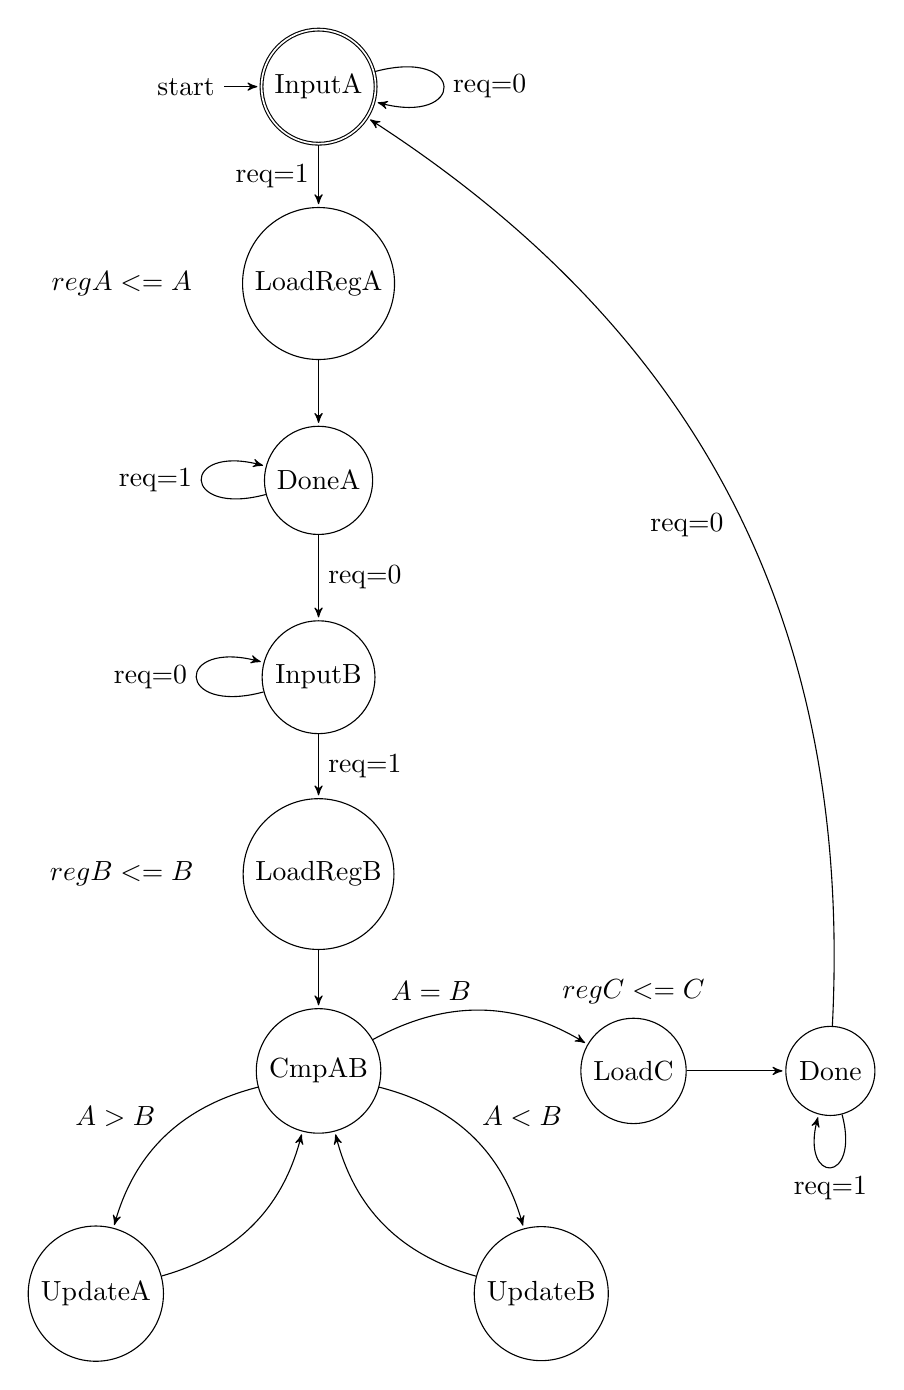
\begin{tikzpicture}[>=stealth',shorten >=1pt,auto,node distance=2.5cm]

  \node[initial,state,accepting]	(InputA) {InputA};
  \node[state]			(LoadRegA) [below of=InputA] {LoadRegA};
  \node [left of=LoadRegA] {$regA<= A$};
  \node[state]			(DoneA) [below of=LoadRegA] {DoneA};
  \node[state]			(InputB) [below of=DoneA] {InputB};
  \node[state]			(LoadRegB) [below of=InputB] {LoadRegB};
  \node [left of=LoadRegB] {$regB<= B$};
  \node[state]			(CmpAB) [below of=LoadRegB] {CmpAB};
  \node[state]			(UpdateA) [below left of=CmpAB, node distance=4 cm] {UpdateA};
  \node[state]			(UpdateB) [below right of=CmpAB, node distance=4 cm] {UpdateB};
  \node[state]			(LoadC)  [ right of=CmpAB, node distance=4 cm] {LoadC};
  \node [above of=LoadC, node distance=1 cm] {$regC<= C$};
  \node[state]			(Done) [right of=LoadC] {Done};


 \path[->]
 (InputA) 
	 edge [loop right] node {req=0} (InputA)
	 edge node  [left] {req=1} (LoadRegA)
 (LoadRegA)
	 edge  node {} (DoneA)
 (DoneA)
	 edge  [loop left] node {req=1} (LoadRegA)
	 edge  node {req=0} (InputB)
 (InputB)
	 edge  [loop left] node {req=0} (InputB)
	 edge  node {req=1} (LoadRegB)
 (LoadRegB)
	 edge  node {} (CmpAB)

(CmpAB)
	 edge [bend right] node [above  left] {$A>B$} (UpdateA)
	 edge [bend left] node [ above right ] {$A<B$} (UpdateB)
	 edge [bend left] node  [above left] {$A=B$} (LoadC)

(UpdateA)
	 edge [bend right] node {} (CmpAB)
(UpdateB)
	 edge [bend left] node {} (CmpAB)
(LoadC)
	edge node  {} (Done)
(Done)
	 edge  [loop below] node {req=1} (Done)
	edge [bend right] node  {req=0} (InputA)

; % end of \path
	




%  \path[->] (S)  edge [loop above] node {a} (S)
%             edge              node {a} (q1)
%        (q1) edge [bend left]  node {a} (S)
%             edge              node {b} (q2)
%        (q2) edge [loop above] node {b} (q2)
%             edge [bend left]  node {b} (q1);
\end{tikzpicture}
\end{document}